\subsection[Raccogliere e ripulire i dati]{Raccogliere e ripulire i dati}

\begin{frame}

	\frametitle{{\color{GradientDescentDiagramBlue}Raccogliere e ripulire i dati}}

%	\begin{block}{}
		Quando si tratta di dati, \textbf{non esiste una ricetta magica}, come afferma:
		\begin{itemize}
			\item il \textbf{No Free Lunch Theorem} (Wolpert, 1996):\\
				\emph{Non esiste un modello o algoritmo di stima universalmente ottimale}
			\item Ogni modello o algoritmo di stima è basato su uno specifico insieme di ipotesi, che può funzionare bene o meno a seconda dell'applicazione in questione. Ecco perchè è importante acquisire familiarità con molti \textbf{tipi diversi di modelli e metodi di stima}
%			\item Esempio:
%
%			\begin{itemize}
%				\item Supponiamo di disporre di $p=100$ predittori binari
%				\item Il numero delle combinazioni possibili degli input è $2^{100} = 1267650600228229401496703205376$
%				\item Non avremo \emph{mai} un campione che contiene un'osservazione della $Y$ per ognuna di queste possibili combinazioni
%				\item Com'è possibile allora che un modello fornisca una previsione $\hat y$ per ognuna di esse? \emph{Grazie alla struttura che implicitamente il modello impone sui dati}
%				\item A seconda dell'applicazione, la struttura può funzionare o meno\ldots
%			\end{itemize}
		\end{itemize}

		Inoltre anche le funzioni di apprendimento più sofisticate e avanzate non ce la fanno e finiscono per avere pessime prestazioni se non le supportate con quanto segue:
		\begin{itemize}
			\item \textbf{quantità di dati sufficientemente grandi} da essere adeguate all'algoritmo che state utilizzando
			\item \textbf{dati puliti e ben preparati} da utilizzare con il machine learning (secondo il principio GIGO = Garbage In, Garbage Out)
		\end{itemize}
%	\end{block}

%Al di là della quantità dei dati, è comprensibile la necessità della loro pulizia. È un po' come la qualità degli insegnamenti che ricevete a scuola: se gli insegnanti vi insegnano solo cose senza senso, vi presentano esempi sbagliati, passano il tempo a scherzare e, in generale, non prendono seriamente l'insegnamento, i vostri esami non potranno andare granché bene, per quanto possiate essere intelligenti. Lo stesso vale sia per gli algoritmi semplici sia per quelli complessi: se li rifocillate di dati spazzatura, le previsioni prodotte non potranno che essere prive di senso.
%Secondo il principio del garbage in, garbage out (o GIGO, letteralmente “spazzatura dentro, spazzatura fuori”, ossia se elabori spazzatura non puoi che ottenere spazzatura, banale ma assolutamente vero), se i dati sono di cattiva qualità il processo di machine learning ne può risultare seriamente compromesso. Con dati di cattiva qualità si intendono dataset presentanti dati mancanti, valori anomali, intere feature composte di valori distorti, ridondanza di informazioni. In questo capitolo tutti questi problemi vengono affrontati, unitamente alle relative possibili soluzioni.

\end{frame}


\subsubsection[Mappare dati grezzi in features]{Mappare dati grezzi in features}
\begin{frame}

	\frametitle{{\color{GradientDescentDiagramBlue}Raccogliere e ripulire i dati}: mappare dati grezzi in features}

%	\begin{block}{Mappare i dati grezzi in features}
%		I dati di cattiva qualità potrebbero non essere di per sé sbagliati:
%		\begin{itemize}
%			\item dati che non ottemperano agli \textbf{standard}
%			\item \textbf{date scritte in formati non validi}
%			\item \textbf{testo non strutturato} da convertire in variabile categorica
%		\end{itemize}
		All'interno di questa fase di raccolta dobbiamo includere anche il \textbf{feature engineering} ovvero il processo con il quale si trasformano i dati grezzi in un vettore di fetures.
		\newlinedouble
		Molti modelli di machine learning devono rappresentare le features come vettori di numeri reali poiché i valori delle features devono essere moltiplicati per i pesi del modello.

		\begin{figure}[!htbp]
			\centering
			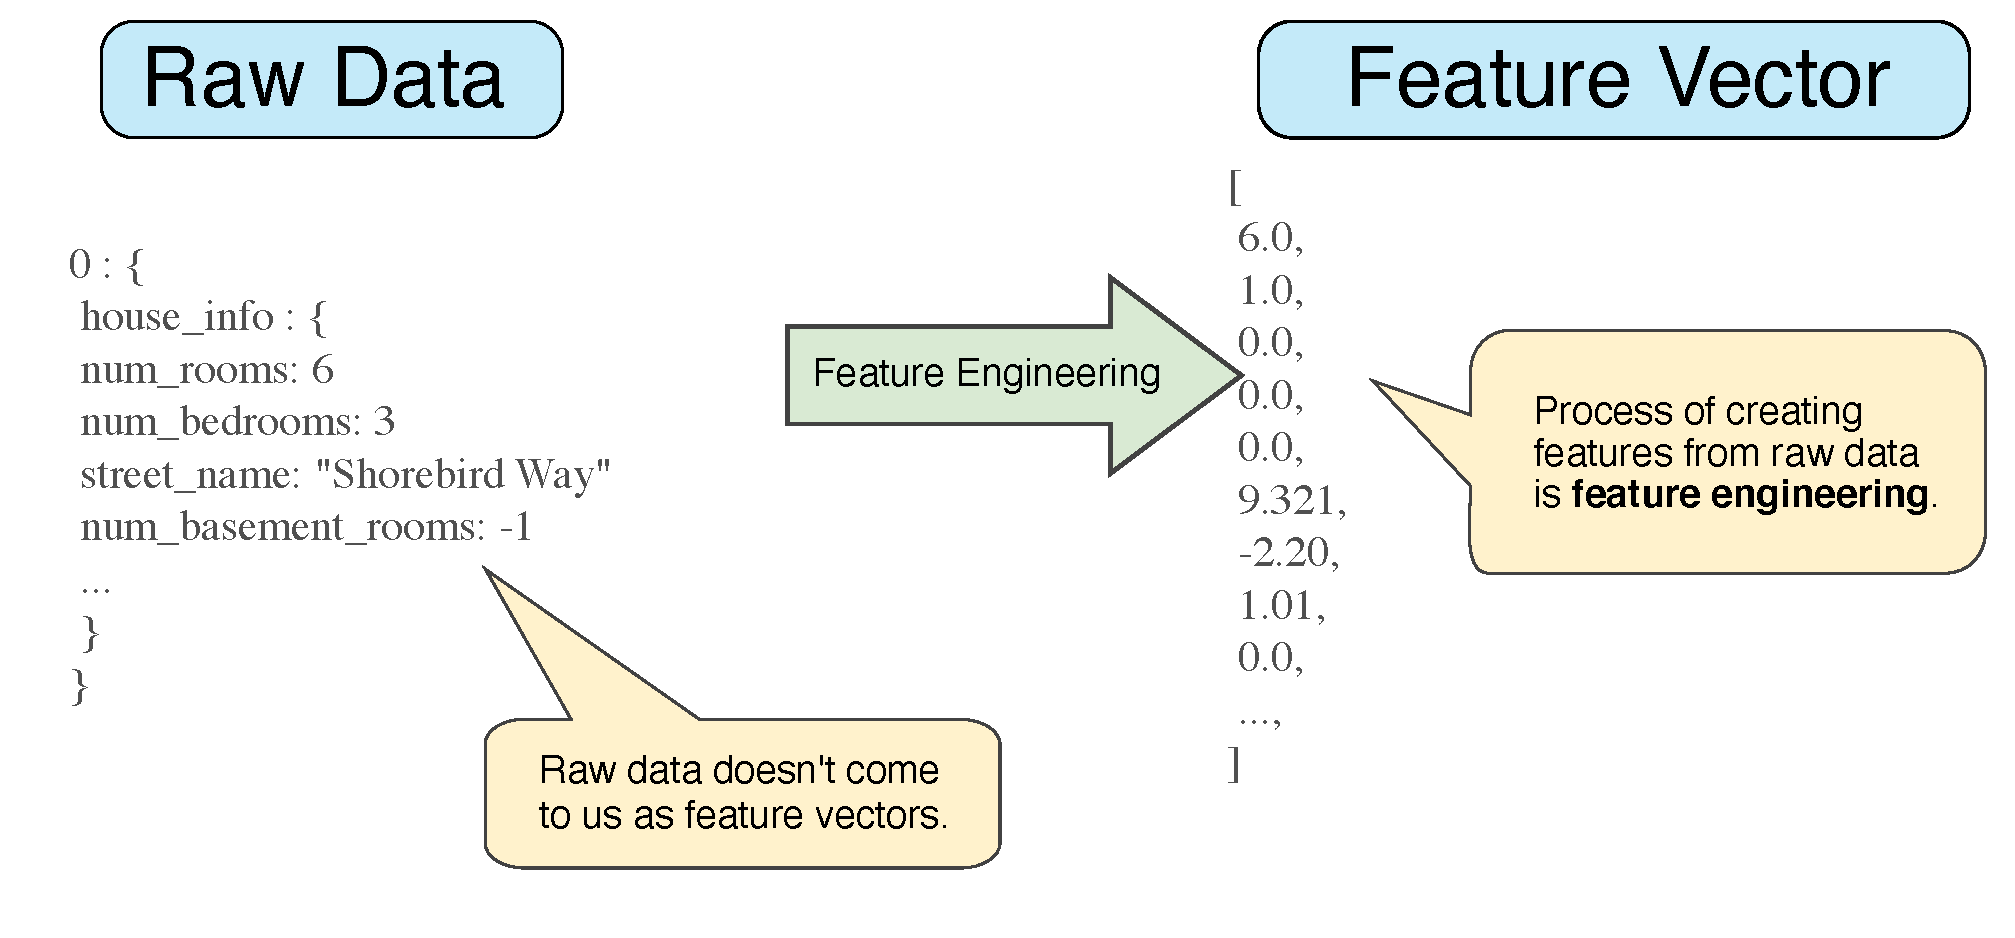
\includegraphics[width=0.75\linewidth]{images/data_prep/feature_engineering_and_data_cleaning/RawDataToFeatureVector.pdf}
					%\caption{Stripe Radar for Fraud Detection}
		\end{figure}
%	\end{block}

\end{frame}


\subsubsection[Mappare valori numerici]{Mappare valori numerici}
\begin{frame}

	\frametitle{{\color{GradientDescentDiagramBlue}Raccogliere e ripulire i dati}: mappare valori numerici}

%	\begin{block}{}
		I dati interi e in virgola mobile non necessitano di una codifica speciale perché possono essere moltiplicati per un peso numerico.\\
		Come suggerito nella figura mostrata, la conversione del valore intero grezzo 6 nel valore della feature 6.0 è procedimento scontato:
		\begin{figure}[!htbp]
			\centering
			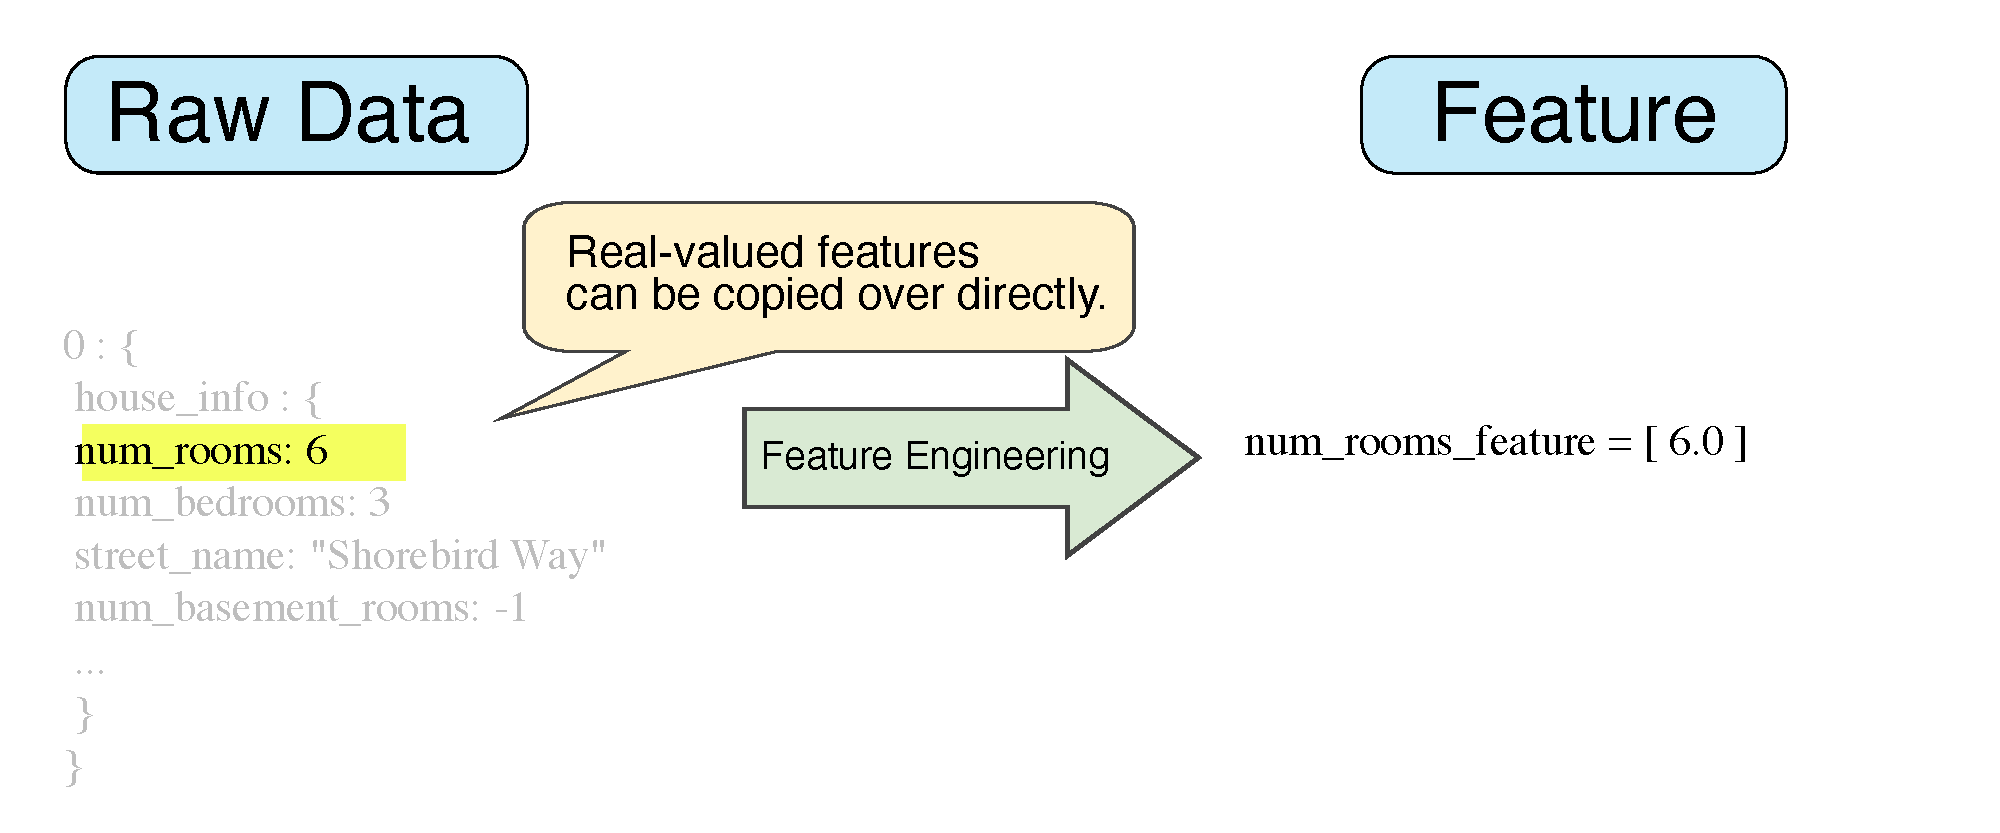
\includegraphics[width=1.0\linewidth]{images/data_prep/feature_engineering_and_data_cleaning/FloatingPointFeatures.pdf}
					%\caption{Stripe Radar for Fraud Detection}
		\end{figure}

%	\end{block}

\end{frame}


\subsubsection[Mappare valori numerici]{Mappare valori categorici}
\begin{frame}

	\frametitle{{\color{GradientDescentDiagramBlue}Raccogliere e ripulire i dati}: mappare valori categorici}

%	\begin{block}{}
		Le features categoriche hanno un insieme discreto di possibili valori.\\
		Ad esempio, potrebbe esserci una feature chiamata \textit{street\_name} con valori che includono:
		\begin{scriptsize}
			\begin{empheq}[box=\fcolorbox{blue!40!black!60}{yellow!10}]{align*}
				\text{\{'Charleston Road', 'North Shoreline Boulevard', 'Shorebird Way', 'Rengstorff Avenue'\}}
			\end{empheq}
		\end{scriptsize}

		Poiché i modelli non possono moltiplicare le stringhe per i pesi appresi, utilizziamo la feature engineering per \textbf{convertire le stringhe in dei valori numerici}.

%	\end{block}

\end{frame}


\begin{frame}

	\frametitle{{\color{GradientDescentDiagramBlue}Raccogliere e ripulire i dati}: mappare valori categorici}

%	\begin{block}{}
		Alcune soluzioni:
		\begin{itemize}
			\item \textbf{mappare il vocabolario in differenti valori interi}. Poiché non tutte le strade del mondo appariranno nel nostro dataset, possiamo raggruppare tutte le altre strade in una categoria chiamata \textit{altro} generico, nota come bucket OOV (out-of-vocabulary)
				\begin{itemize}
					\item[--] questi valori numerici così imposti potrebbero non avere una relazione lineare con la label da predire. Modelli poco flessibili non saranno in grado di utilizzare questa feature in modo adeguato
					\item[--] non è possibile codificare una relazione uno a molti (se ad esempio una casa è ad un incrocio)
				\end{itemize}
			\item \textbf{one-hot encoding}: creare un vettore binario per ogni feature categorica nel nostro modello che rappresenta i valori come segue:
				\begin{itemize}
					\item[--] il vettore varrà 1 in corrispondenza della posizione del vettore che matcha lo specifico valore categorico
					\item[--] 0 su tutti gli altri
				\end{itemize}
			\item \textbf{multi-hot encoding}: simile al \textit{one-hot encoding} ma prevede la possibilità di più di un solo 1 nel vettore
		\end{itemize}



%	\end{block}

\end{frame}


\begin{frame}

	\frametitle{{\color{GradientDescentDiagramBlue}Raccogliere e ripulire i dati}}

	\begin{block}{}

		\begin{figure}[!htbp]
			\centering
			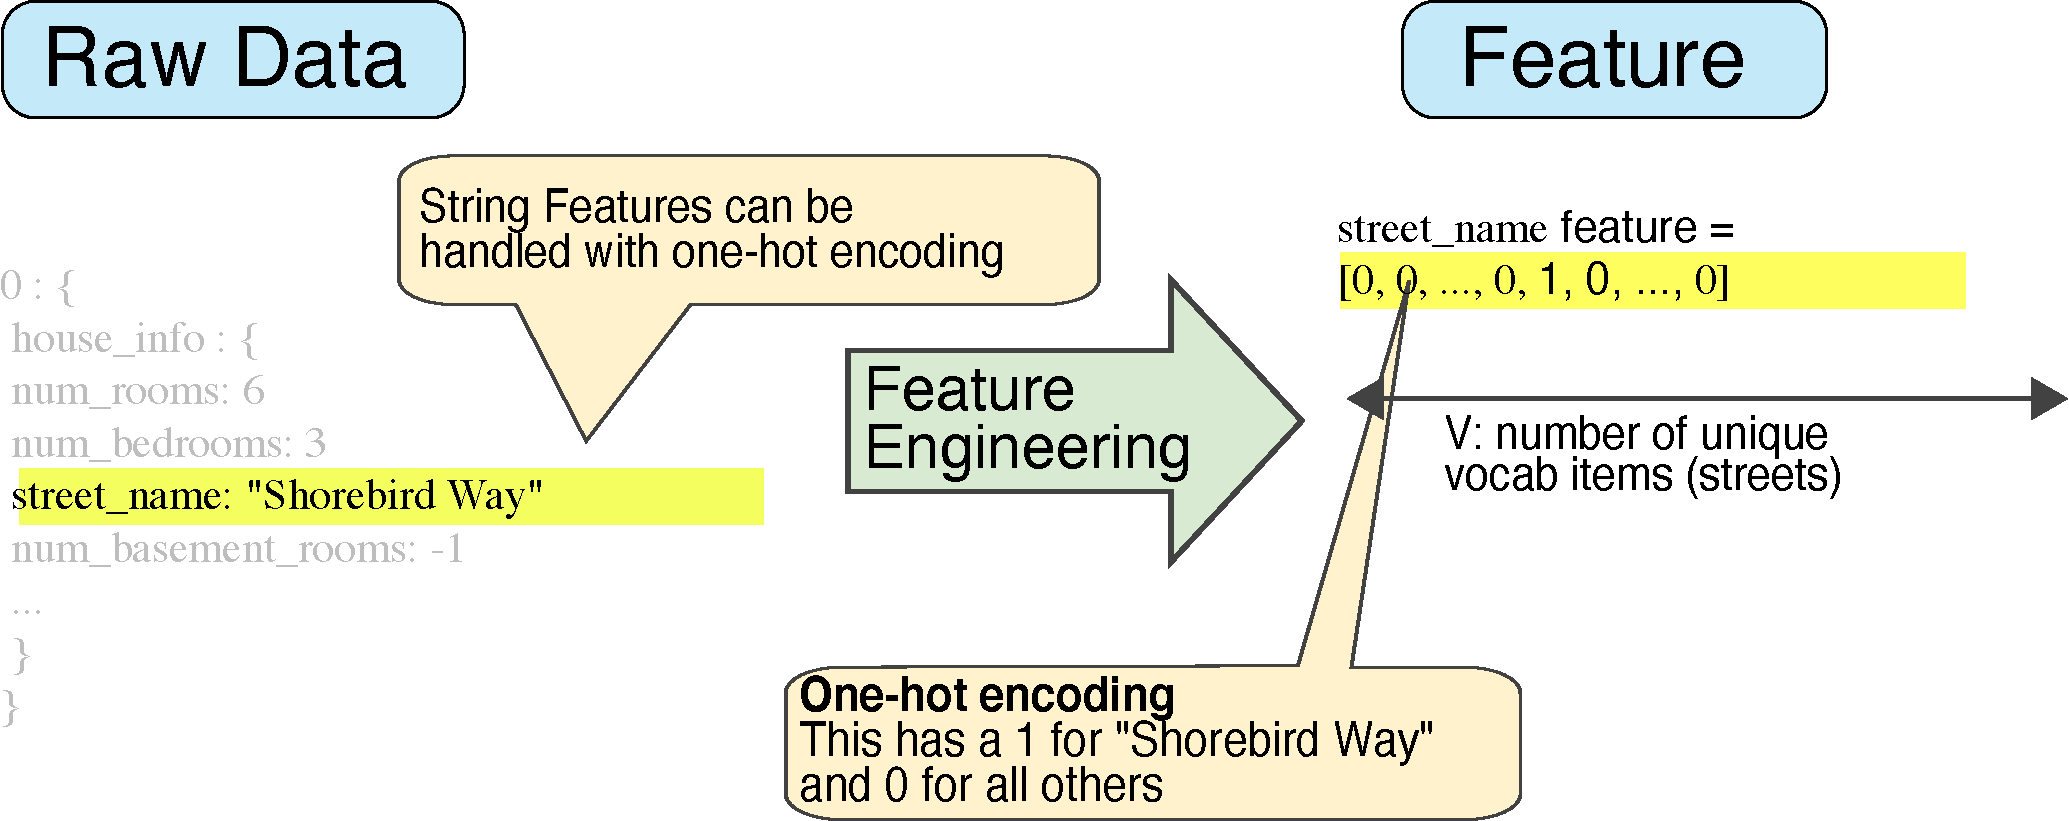
\includegraphics[width=1.0\linewidth]{images/data_prep/feature_engineering_and_data_cleaning/OneHotEncoding.pdf}
					%\caption{Stripe Radar for Fraud Detection}
		\end{figure}

	\end{block}

\end{frame}


\begin{frame}

	\frametitle{{\color{GradientDescentDiagramBlue}Raccogliere e ripulire i dati}}

	\begin{block}{Alcune linee guida per costruzione e l'uso di buone features}
		\begin{itemize}
			\item evitare valori di elementi discreti usati raramente
			\item ogni feature dovrebbe avere un significato chiaro e il più ovvio possibile
			\item non mischiare \textbf{magic numbers} con dati reali
			\item la definizione di una feature non dovrebbe cambiare nel tempo
		\end{itemize}
	\end{block}

\end{frame}


\subsubsection[Mappare valori numerici]{Ripulire i dati: lo scrubbing}
\begin{frame}

	\frametitle{{\color{GradientDescentDiagramBlue}Raccogliere e ripulire i dati}}

	\begin{block}{Ripulire i dati: lo scrubbing}
		Fino ad ora, abbiamo ipotizzato che tutti i dati utilizzati per l'addestramento e il test fossero affidabili.\\
		\vspace{1mm}
		Nella vita reale, molti esempi dataset non sono affidabili a causa di uno o più dei seguenti motivi:

		\begin{itemize}
			\item \textbf{valori omessi}. Ad esempio, una persona ha dimenticato di inserire un valore per l'età di una casa
			\item \textbf{esempi duplicati}. Ad esempio, un server ha erroneamente caricato due volte gli stessi log
			\item \textbf{etichette sbagliate}. Ad esempio, una persona ha erroneamente etichettato l'immagine di una quercia come un acero
			\item \textbf{valori di feature errati}. Ad esempio, qualcuno ha digitato una cifra in più
		\end{itemize}

	\end{block}

\end{frame}
